%%%%%%%%%%%%%%%%%%%%%%%%%%%%%%%%%%%%%%%%%%%%%%%%%%%%%%%%%%%%%%%%%%
%%%%%%%% ICML 2010 EXAMPLE LATEX SUBMISSION FILE %%%%%%%%%%%%%%%%%
%%%%%%%%%%%%%%%%%%%%%%%%%%%%%%%%%%%%%%%%%%%%%%%%%%%%%%%%%%%%%%%%%%

% Use the following line _only_ if you're still using LaTeX 2.09.
%\documentstyle[icml2010,epsf,natbib]{article}
% If you rely on Latex2e packages, like most moden people use this:
\documentclass{article}
\usepackage[utf8]{inputenc}

% For figures
\usepackage{graphicx} % more modern
%\usepackage{epsfig} % less modern
\usepackage{subfigure} 

% For citations
\usepackage{natbib}

% For algorithms
\usepackage{algorithm}
\usepackage{algorithmic}

% As of 2010, we use the hyperref package to produce hyperlinks in the
% resulting PDF.  If this breaks your system, please commend out the
% following usepackage line and replace \usepackage{icml2010} with
% \usepackage[nohyperref]{icml2010} above.
%\usepackage{hyperref}

% Packages hyperref and algorithmic misbehave sometimes.  We can fix
% this with the following command.
\newcommand{\theHalgorithm}{\arabic{algorithm}}

% Employ the following version of the ``usepackage'' statement for
% submitting the draft version of the paper for review.  This will set
% the note in the first column to ``Under review.  Do not distribute.''
% \usepackage{icml2010} 
% Employ this version of the ``usepackage'' statement after the paper has
% been accepted, when creating the final version.  This will set the
% note in the first column to ``Appearing in''
%\usepackage[accepted, nohyperref]{icml2010}
\usepackage[nohyperref]{icml2010}


% The \icmltitle you define below is probably too long as a header.
% Therefore, a short form for the running title is supplied here:
\icmltitlerunning{Number recognition for use in a Sudoku solver}


% custom imports
\usepackage{amsmath}

\begin{document} 

\twocolumn[
\icmltitle{Number recognition for use in a Sudoku solver}

% It is OKAY to include author information, even for blind
% submissions: the style file will automatically remove it for you
% unless you've provided the [accepted] option to the icml2010
% package.
\icmlauthor{Ralf Vogler}{voglerr@in.tum.de}
\icmladdress{TU München}
\icmlauthor{Simon Grötzinger}{groetzin@in.tum.de}
\icmladdress{TU München}

% You may provide any keywords that you 
% find helpful for describing your paper; these are used to populate 
% the "keywords" metadata in the PDF but will not be shown in the document
\icmlkeywords{neural network, svm, logistic regression, synthetic data generation, machine learning}

\vskip 0.3in
]

\begin{abstract}
The goal of this work is to implement number recognition for a Soduko solver.
First we will describe the generation of synthetic data, in this case labelled images of numbers.
Then we compare different machine learning techniques for supervised learning using the generated data.
Once the training is complete, images of real Sudokus are captured using a webcam and preprocessed to be predicted by the learned models. We evaluate the different approaches by analyzing their performance on different data sets.
\end{abstract}

\section{Introduction}
Number and letter recognition is key in many real-world applications. Digitalizing print media, automated sorting of letters, or recognition of signs in robotics or driver assistance systems require well performing algorithms for character recognition. In the following we analyze the performance of different techniques for number recognition, namely Neural Networks (NN), Support Vector Machines (SVM) and Logistic Regression (LR), by using them in an automated Sudoku solver.

\section{Overview}
Figure \ref{fig:overview} shows the basic data flow and the participating data manipulators. First of all we generate data by sampling position, rotation, size and color of a number and place it based on these values on a white 20x20 pixel image. Examples of 9 such generated images are shown in Figure \ref{fig:generated_numbers}.The corresponding labels are defined by the name of the folder the images are stored in.
\begin{figure}[ht]
	\centerline{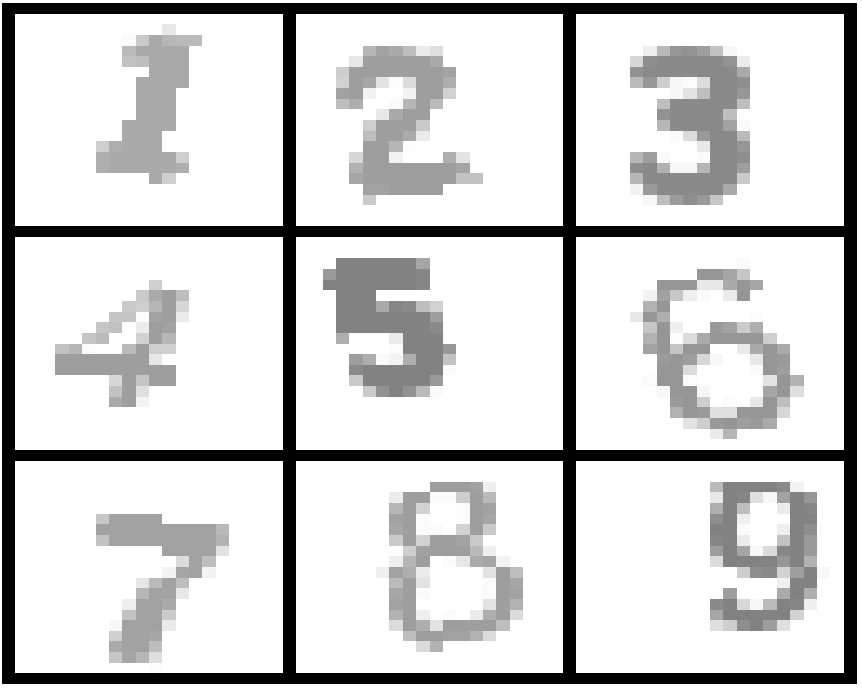
\includegraphics[scale=0.25]{../examples}}
	\caption{Examples of generated numbers}
	\label{fig:generated_numbers}
\end{figure}
These images are preprocessed (applying greyscale) by an octave script and written to an input matrix and a target vector. All pixels of one image are encoded in one row of the input matrix and the corresponding label is stored in the row of the target vector. The data is dumped to a ``cache.mat'' file which allows us to apply many different tools and programming languages to the dataset. In our case we use it in python and octave.
% trim=l b r t
\begin{figure}[ht]
	\centerline{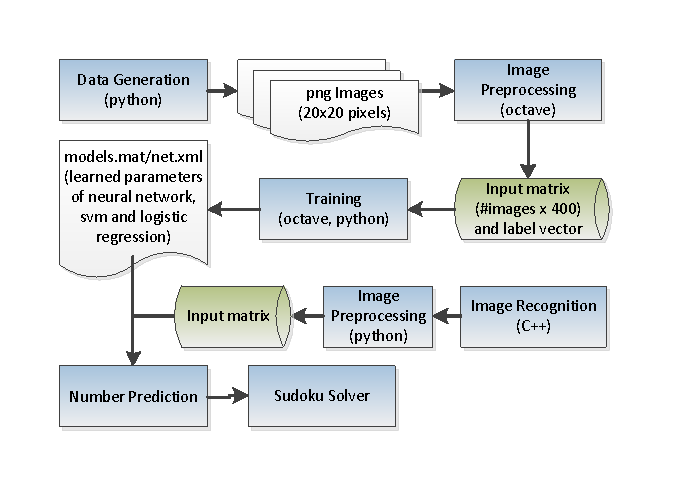
\includegraphics[width=\columnwidth, trim=25 30 25 30]{../overview}}
	\caption{Overview}
	\label{fig:overview}
\end{figure}
The input matrix $X^{n\text{x}400}$ and the target vector $y$ are the inputs for training NN, SVM and LR, as described in Section \ref{training}. After training, the learned models/parameters are saved in ``.mat'' files that can be loaded by the number prediction. The other input for number prediction is an input matrix of the same form as $X$ with a row entry for each Sudoku field that was detected to contain a number. This implies that we do not train our models to detect empty fields. We could detect empty fields with high accuracy by performing some preprocessing steps on the images (filling borders, adjusting thresholds etc.) thus applying a machine learning technique does not seem appropriate for this task.

\section{Training}
\label{training}
\subsection{Neural Network}
Applying a NN seems promising as it was already successfully applied to the quite similar problem of detecting handwritten digits.\footnote{http://www.ml-class.org} For the NN we choose a simple architecture with 25 hidden sigmoidal units (+ bias unit), as shown in figure \ref{fig:nn}. The size of the input layer is 400 (given by the 20 x 20 pixel images) and the size of the output layer is defined by the number of classes, in this case the numbers 1 to 9. This simple architecture turned out to perform pretty well compared to more complex ones with a higher number of hidden layers. Training is performed with error backpropagation, thus minimizing the error function
\begin{align*}
& E(w) = \sum_{n=1}^N E_n(w)\\
\text{with}~~E&_n(w) = \frac{1}{2}\sum_k (y_{nk}-t_{nk})\\
\text{and}~~~~~&~~~y_k = \sum_i w_{ki}x_{i}\\
\end{align*}
subject to $w$.
\begin{figure}[ht]
	\centerline{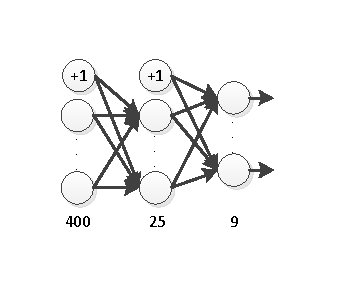
\includegraphics[width=\columnwidth, trim=0 30 0 30]{../nn}}
	\caption{Neural Network with one hidden layer}
	\label{fig:nn}
\end{figure}
For NNs we test two implementations. On the one hand we use a partly self-developed octave code for two-layer NNs which was written as part of the stanford machine learning course\footnote{http://www.ml-class.org}, on the other hand we include PyBrain \cite{schaul2010pybrain} for comparison and easier evaluation of more sophisticated network architectures. To find a good value for the regularization parameter $\lambda$ we perform a grid search with k-fold cross-validation which gives us a good performance when choosing $\lambda = 1$.

\subsection{Support Vector Machines}
The next technique we apply to the discussed problem are Support Vector Machines \cite{Bishop200608} which try to solve the following optimization problem:
\begin{align*}
\min_{w,b} &~~ \frac{1}{2}||w||^2 + C \sum_{i=1}^{n} \xi_i\\
\text{subject to } &~~ y_i(w^T \phi(x_i) + b) - 1 + \xi_i \ge 0\\
\text{and} &~~ \xi_i \ge 0.
\end{align*}
Using a radial basis function (RBF) as kernel we perform a grid search over $C$ and $\gamma$ to find those parameters that provide highest accuracy on the test set. We use the open source library ``libsvm'' \cite{chang2011libsvm} wrapped by some octave scripts for setting up data sets and performing grid search with k-fold cross-validation. Grid search with cross validation resulted in accuracies illustrated in Figure \ref{fig:svm_grid_search}. We can see that there is a certain area of $(C,\gamma)$ pairs which provide an accuracy close to $100\%$. To prevent overfitting we decide to choose $C$ and $\gamma$ by cross checking good pairs against another validation set. Further refinement results in the following values $C = 20$ and $\gamma = 0.1$.
\begin{figure}[ht]
	\centerline{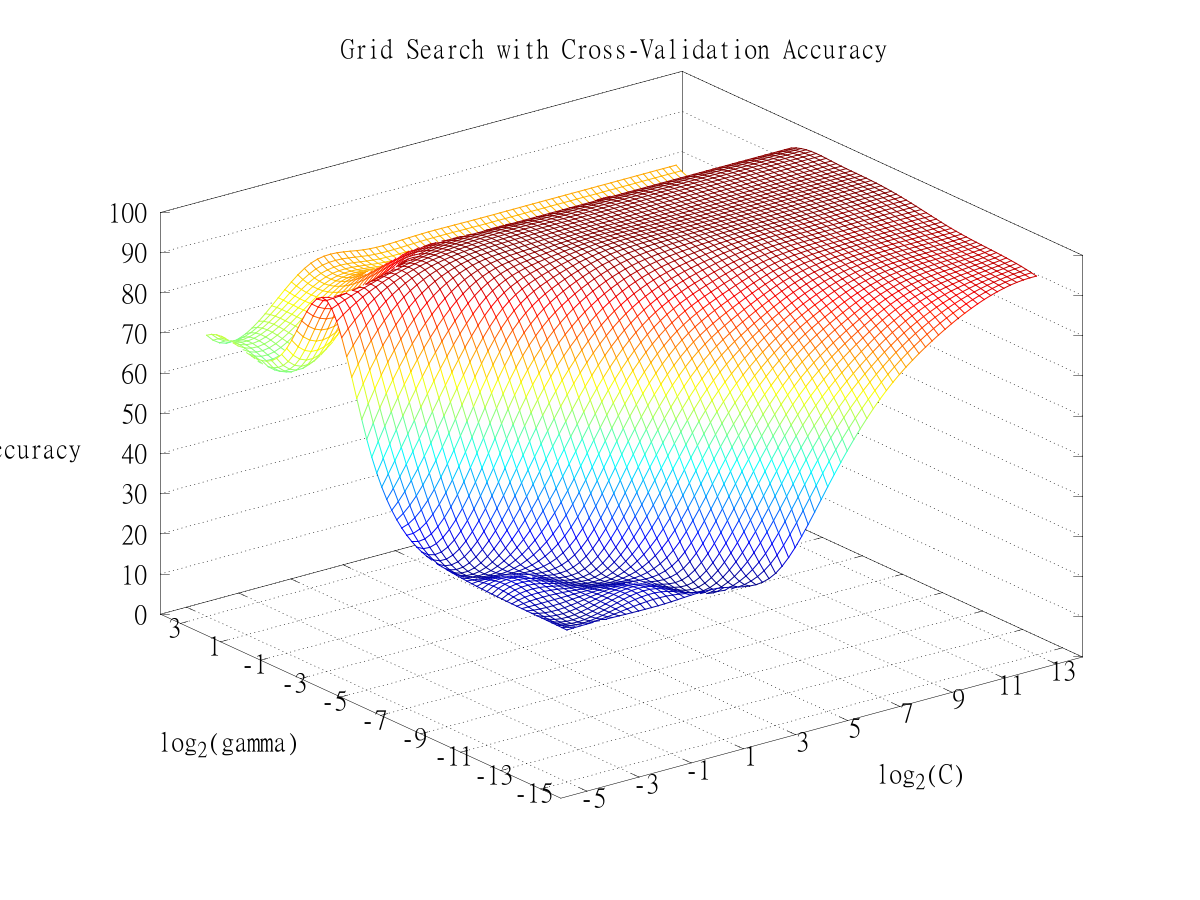
\includegraphics[scale=0.20, trim=0 0 10 0]{../gridSearchSVMPlot}}
	\caption{}
	\label{fig:svm_grid_search}
\end{figure}

\subsection{Logistic Regression}
Finally we apply Logistic Regression to the datasets. Again we use a (vectorized) octave implementation for learning and prediction. Therefore we minimize the (regularized) error function
\begin{align*}
E(w) &= \frac{1}{n}(-y^T ln(\Phi w) + (1-y^T)ln(1-\Phi w))\\
&~~~+\frac{\lambda}{2n}w^Tw
\end{align*}
with respect to $w$. Minimization is performed by an algorithm\footnote{http://sprinkler.googlecode.com/svn/trunk/\\regression/fmincg.m} that was provided during the stanford machine learning course. Grid search and k-fold cross-validation recommend a value for the regularization parameter $\lambda$.

\section{Image Recognition and Preprocessing}
Image recognition is written in C by extensive use of the open source library OpenCV\footnote{http://opencv.willowgarage.com/wiki/}. Images captured by the webcam are continously analyzed to find a Sudoku square. Images are transformed to greyscale, then an adaptive threshold algorithm is used to preprocess the image for contour detection by OpenCV. OpenCV returns a list of contours which are further checked for certain criteria like having four corners or being of certain size. Since the contours are not detected precise enough lines are fitted through six checkpoints on each edge in order to achieve subpixel accuracy. The content enclosed by the corners is perspectively warped to fit a predefined square size. Finally, the thresholded Sudoku field is saved to disk. A python script is then used to split the whole field into 9x9 subfields with each subfield being flood filled around the corners for noise reduction. The format of the subfields now equals to the one provided by the generated images which allows us to apply the trained NN/SVM/LR models and, finally, apply a Sudoku solver.

\section{Evaluation}
To evaluate the performance of different approaches we define the following data sets:
\begin{itemize}
\item D1: 4500 generated images
\item D2: $\sim$ 1000 gathered images
\item D3: D1 $\cup$ D2
\item DVal: images of some newly captured Sudoku
\end{itemize}

\begin{table}[t]
\caption{Classification accuracies for Neural Network, SVM and Logistic Regression on different data sets. All values are rounded averages!}
\label{sample-table}
\vskip 0.15in
\begin{center}
\begin{small}
\begin{sc}
\begin{tabular}{lccccc}
\hline
\abovespace\belowspace
Data & NN & pyNN & SVM & LR & Winner \\
\hline
\abovespace
D1 		& 78.0 &  & 100 & 80.80 & ?\\
D2		& 93.4 & 95.94 & 94.41 & 91.36 & pyNN\\
D3		&  & & & & ? \\
\belowspace
DVal	& 89.3 & 88.1 & 92.7 & 85.3 & SVM\\
\hline
\end{tabular}
\end{sc}
\end{small}
\end{center}
\vskip -0.1in
\end{table}
As expected, on data sets D1, D2 and D3 all approaches performed pretty well as they were used for training. DVal is the data set that contains completely new images that were never used for training by any of the models. Thus, these values are the most interesting ones for evaluation. SVM and NN have comparable performance. Yet, the SVM is cheaper to train which is why applying an SVM seems more appropriate than using a NN. LR is outperformed by the other approaches but predicts with acceptable performance and requires less effort to train.

\section{Future Work}
Several ideas arose during this project. A first step could be to implement online learning to empower the models to evolute over time and increase their accuracy with more Sudokus being scanned. When detecting new Sudokus it turned out that empty field detection was not as reliable as expected, especially when light conditions were bad. Improving this part of the system or maybe doing it from a machine learning point of view (adding a new label for empty fields) might be a good idea. Another improvement of the systems accuracy could be achieved by including information of the Sudoku solver into field prediction. The solver could inform about impossible field combinations forcing the number prediction script to maybe choose a less probable number combination from the model point of view, yet, being a possible one.

\bibliography{paper}
\bibliographystyle{icml2010}

\end{document}  


